% Figure: CPG vs training-set size, with validation MSE on a secondary axis.
% Source data: results/dmc_acrobot/cpg_sweep.json (cell-by-cell pooled n=150).
%
% Numbers (kept here so the figure is self-checking against the table):
%   data=200    val_mse=0.0651  CPG=+0.267  AC 95% CI [+0.191, +0.335]
%   data=2000   val_mse=0.0233  CPG=+0.267  AC 95% CI [+0.191, +0.335]
%   data=20000  val_mse=0.00042 CPG=+0.267  AC 95% CI [+0.191, +0.335]
%
% The CPG whiskers are asymmetric to match the AC CI exactly:
%   lower whisker = 0.267 - 0.191 = 0.076
%   upper whisker = 0.335 - 0.267 = 0.068
% (the plus-4 adjustment offsets the AC midpoint 0.263 from the raw CPG
% 0.267, so the interval is not symmetric around the point estimate).
\begin{figure}[t]
  \centering
  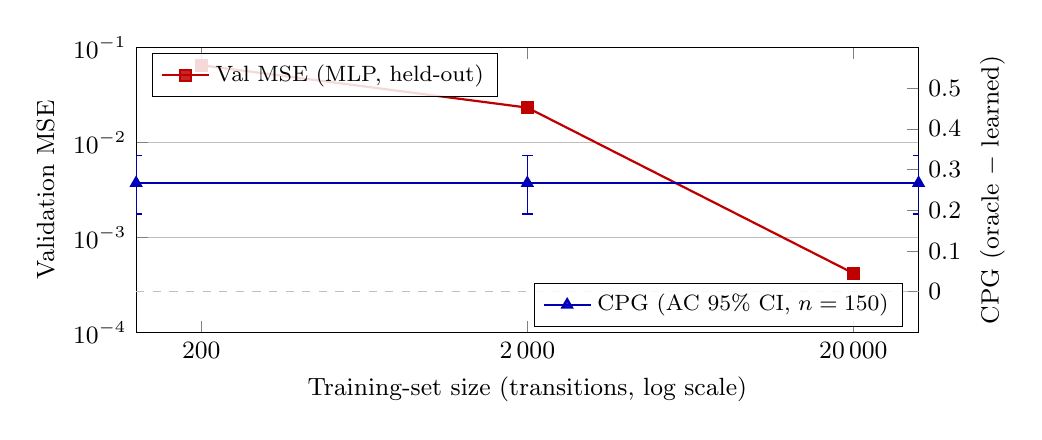
\begin{tikzpicture}
    \pgfplotsset{
      every axis/.append style={
        width=0.95\columnwidth,
        height=5.2cm,
        font=\small,
      },
    }
    \begin{axis}[
        xmode=log, log basis x=10,
        xtick={200, 2000, 20000},
        xticklabels={$200$, $2\,000$, $20\,000$},
        xlabel={Training-set size (transitions, log scale)},
        ymode=log, log basis y=10,
        axis y line*=left,
        ylabel={Validation MSE},
        ymin=1e-4, ymax=1e-1,
        ytick={1e-4, 1e-3, 1e-2, 1e-1},
        ymajorgrids=true,
        legend cell align=left,
        legend style={
          at={(0.02, 0.98)}, anchor=north west,
          fill=white, fill opacity=0.85, draw opacity=1,
          text opacity=1, font=\footnotesize,
        },
      ]
      \addplot[color=red!75!black, mark=square*, thick]
        coordinates {(200, 0.0651) (2000, 0.0233) (20000, 0.00042)};
      \addlegendentry{Val MSE (MLP, held-out)}
    \end{axis}
    \begin{axis}[
        xmode=log, log basis x=10,
        xmin=200, xmax=20000,
        axis y line*=right,
        axis x line=none,
        ylabel={CPG (oracle $-$ learned)},
        ymin=-0.1, ymax=0.6,
        ytick={0, 0.1, 0.2, 0.3, 0.4, 0.5},
        legend cell align=left,
        legend style={
          at={(0.98, 0.02)}, anchor=south east,
          fill=white, fill opacity=0.85, draw opacity=1,
          text opacity=1, font=\footnotesize,
        },
      ]
      \draw[dashed, gray!50] (axis cs:200, 0) -- (axis cs:20000, 0);
      \addplot+[
          color=blue!70!black, mark=triangle*, thick,
          error bars/.cd,
          y dir=both,
          y explicit,
        ]
        table[
          x=x, y=y,
          y error plus=eplus,
          y error minus=eminus,
          row sep=\\,
        ]{
          x     y     eplus  eminus \\
          200   0.267 0.068  0.076  \\
          2000  0.267 0.068  0.076  \\
          20000 0.267 0.068  0.076  \\
        };
      \addlegendentry{CPG (AC 95\% CI, $n = 150$)}
    \end{axis}
  \end{tikzpicture}
  \caption{Validation MSE (red, log scale, left axis) drops by $\sim\!150\times$ across the training-set sweep while CPG (blue, right axis) stays exactly flat at $+0.267$ with the same Agresti--Caffo $95\%$ CI $[+0.191, +0.335]$ in every cell. Predicting better did not plan better. Numbers from \texttt{results/dmc\_acrobot/cpg\_sweep.json}.}
  \label{fig:cpg_vs_data}
\end{figure}
